
\chapter{Resultados y pruebas}

En las siguientes secciones se expondrán los resultados que se han obtenido tras usar la nueva nomenclatura implementada y los cambios en el sistema de representación. Se describirán también las pruebas llevadas a cabo para validar todo este proceso.

\section{Nomenclatura canónica}

Para la canonización, se muestra en la siguiente Tabla \ref{tab:canon_smiles} una comparativa entre el SMILES original, el SMILES canónico obtenido utilizando el algoritmo de OpenBabel (\textit{canonicalLabels}), y el SMILES canónico obtenido utilizando el algoritmo implementado. Se agrupan en bloques de 3, siendo cada línea con separación cada uno de los SMILES en el orden comentado. No aparecen todas las moléculas del dataset en la tabla ya que se haría excesivamente grande; se han introducido algunas de manera aleatoria para ver los cambios entre las nomenclaturas. Las demás estarán disponibles para su consulta en GitHub en la carpeta \textit{`output'}.

\begin{longtable}{m{0.3cm}>{\arraybackslash}m{11.5cm}}
\caption{Se muestran los SMILES en este orden: original, openbabel, implementación propia. Los Id hacen referencia al Anexo \ref{apend:pagina_tabla_intro_grande}.}\\
\toprule
 \textbf{Id} & \textbf{SMILES} \\ \midrule
\endfirsthead

\multicolumn{2}{c}%
{{\bfseries \tablename\ \thetable{} -- Continuación de la página anterior}} \\
\toprule
\textbf{Id} & \textbf{SMILES} \\ \midrule
\endhead

\hline \multicolumn{2}{r}{{Continúa en la siguiente página}} \\
\endfoot

\hline
\endlastfoot

% Mol 3
 % \multirow{3}{*}{3} & %$\rightarrow$ &
 & [Cl-][Pd+2]123([Cl-])[CH]=4CC[CH]3=[CH]2CC[CH]41      \\ [0.3cm]
 3 & [Cl-][Pd+2]123([Cl-])[CH]4=[CH]3CC[CH]2=[CH]1CC4               \\ [0.3cm]
 & [Pd+2]123([Cl-])([Cl-])[CH]4=[CH]3CC[CH]1=[CH]2CC4               \\ 
\midrule

% Mol 4
 % \multirow{3}{*}{4} & %$\rightarrow$ &
 & [Cl-][Pd+2]1([C-]=2C=CC=CC2C=3C=CC=CC3[N]1(C)C)[PH](C4C C5CCC4C5)C6CC7CCC6C7      \\ [0.5cm]
 4 & [Cl-][Pd+2]1([C-]2=C(C=CC=C2)c2ccccc2[N]1(C)C)[PH](C1C C2CCC1C2)C1CC2CCC1C2               \\ [0.5cm]
 & [Pd+2]1([Cl-])([PH](C2CC3CC2CC3)C2CC3CC2CC3)[C$-$]2=C(C= CC=C2)c2c([N]1(C)C)cccc2              \\ 
\midrule

% Mol 5
 % \multirow{3}{*}{5} & %$\rightarrow$ &
 & OC=1C=CC=2C(=[N](O)[Pd+2]3([Cl-][Pd+2]4([Cl-]3)[C-]=5C=C (O)C=CC5C(=[N]4O)C)[C-]2C1)C      \\ [0.7cm]
 5 & OC1=C[C-]2=C(C=C1)C(=[N](O)[Pd+2]12[Cl$-$][Pd+2]2([Cl$-$]1)[C$-$] 1=C(C=CC(=C1)O)C(=[N]2O)C)C               \\ [0.7cm]
 & [Pd+2]12([C-]3=C(C(C)=[N]2O)C=CC(O)=C3)[Cl$-$][Pd+2]2([Cl$-$]1) [C$-$]1=C(C(C)=[N]2O)C=CC(O)=C1               \\ 
\midrule



% Mol 7
 % \multirow{3}{*}{7} & %$\rightarrow$ &
 & O=S(=O)([NH-][Pd+4]12([F-])([C-]=3C=CC=CC3C(C)(C)[CH2$-$]1) [N]=4C=CC=CC4C=5C=CC=C[N]52)C6=CC=C(C=C6)C      \\ [0.7cm]
 7 & O=S(=O)([NH-][Pd+4]12([F-])([C-]3=C(C=CC=C3)C(C)(C)[CH2$-$]1) [N]1=C(C=CC=C1)C1=[N]2C=CC=C1)c1ccc(cc1)C               \\ [0.7cm]
 & [Pd+4]12([F-])([CH2-]C(C)(C)C3=[C-]2C=CC=C3)([NH-]S(=O)(=O)c2 ccc(C)cc2)[N]2=C(C=CC=C2)C2=[N]1C=CC=C2               \\ 
\midrule



% Mol 15
 % \multirow{3}{*}{15} & %$\rightarrow$ &
 & [Cl-][Au+][P](C=1C=CC=CC1C=2C=CC=CC2)(C(C)(C)C)C(C)(C)C      \\ [0.5cm]
 15 & [Cl-][Au+][P](c1ccccc1c1ccccc1)(C(C)(C)C)C(C)(C)C               \\ [0.5cm]
 & [Au+]([Cl-])[P](C(C)(C)C)(C(C)(C)C)c1ccccc1c1ccccc1               \\ 
\midrule


% Mol 18
 % \multirow{3}{*}{18} & %$\rightarrow$ &
 & [Cl-][Au+][P](C=1C=CC=CC1C=2C(=CC(=CC2C(C)C)C(C)C)C(C) C)(C3CCCCC3)C4CCCCC4      \\ [0.5cm]
 18 & [Cl-][Au+][P](c1ccccc1c1c(cc(cc1C(C)C)C(C)C)C(C)C)(C1CCCC C1)C1CCCCC1               \\ [0.5cm]
 & [Au+]([Cl-])[P](C1CCCCC1)(C1CCCCC1)c1ccccc1c1c(C(C)C)cc(C (C)C)cc1C(C)C               \\ 
\midrule

% Mol 19
 % \multirow{3}{*}{19} & %$\rightarrow$ &
 & [Cl-][Au+][P](C=1C=CC=CC1C2=C(OC(C)C)C=CC=C2OC(C)C) (C=3C=CC=CC3C4=C(OC(C)C)C=CC=C4OC(C)C)C5CCCCC5     \\ [0.7cm]
 19 & [Cl-][Au+][P](c1ccccc1c1c(OC(C)C)cccc1OC(C)C)(c1c cccc1c1c(OC(C)C)cccc1OC(C)C)C1CCCCC1               \\ [0.7cm]
 & [Au+]([Cl-])[P](C1CCCCC1)(c1ccccc1c1c(OC(C)C)ccc c1OC(C)C)c1ccccc1c1c(OC(C)C)cccc1OC(C)C               \\ 
\midrule



% Mol 24
 % \multirow{3}{*}{24} & %$\rightarrow$ &
 & Cl[Au]=C1N(C=CN1C=2C(=CC(=CC2C)C)C)C=3C(=CC(=CC3C)C)C      \\ [0.3cm]
 24 & Cl[Au]=c1n(ccn1c1c(cc(cc1C)C)C)c1c(cc(cc1C)C)C               \\ [0.3cm]
 & [Au](Cl)=c1n(c2c(C)cc(C)cc2C)ccn1c1c(C)cc(C)cc1C               \\ 
\midrule


% Mol 28
 % \multirow{3}{*}{28} & %$\rightarrow$ &
 & O\#C[Fe+2]1234([I-])(C\#O)[CH]=5[CH]4=[CH]3[CH-]2[CH]51      \\ [0.3cm]
 28& [O]\#C[Fe+2]1234([I-])(C\#[O])[CH]5=[CH]4[CH-]3[CH]2=[CH]15               \\ [0.3cm]
 & [Fe+2]1234([I-])(C\#[O])(C\#[O])[CH-]5[CH]3=[CH]2[CH]1=[CH]45         \\      
\midrule

% Mol 30
 % \multirow{3}{*}{30} & %$\rightarrow$ &
 & [I-][Ir+3]12345([I-][Ir+3]6789([I-])([I-]1)C=\%10(C)C9(C)=C8(C)[C$-$] 7(C)C\%106C)C=\%11(C)C5(C)=C4(C)[C-]3(C)C\%112C      \\ [0.7cm]
 30 & [I-][Ir+3]12345([I-][Ir+3]6789([I-])([I-]1)[C]1(=[C]9([C$-$]8([C]7(=[C]61 C)C)C)C)C)[C]1(=[C]5([C-]4([C]3(=[C]21C)C)C)C)C               \\ [0.7cm]
 & [Ir+3]12345([I-])([C-]6(C)[C]1(C)=[C]3(C)[C]4(C)=[C]26C)[I$-$] [Ir+3]1234([I-]5)([I-])[C]5(C)=[C]3(C)[C]2(C)=[C]1(C)[C-]45C               
% \midrule

\label{tab:canon_smiles}
\end{longtable}

\pagebreak

Con esta solución en donde se organiza el SMILES según sus ramificaciones, se ha intentado también dar un enfoque al canonizado orientado a la representación 2D. De esta manera, podemos visualizar ambos e identificar claramente la correspondencia entre una porción contigua del SMILES con una sección de la representación gráfica. Así, se recorren primero todos los vecinos con menor longitud de un átomo hasta cerrar esa rama antes de pasar a la siguiente, obteniendo un SMILES más limpio y evitando que átomos individuales se queden al final de ramificaciones muy largas. Esto se puede ver en la Figura \ref{fig:smiles_vs_dibujo}.

\begin{figure}[h!]
\begin{subfigure}{.9\textwidth}
  \centering
  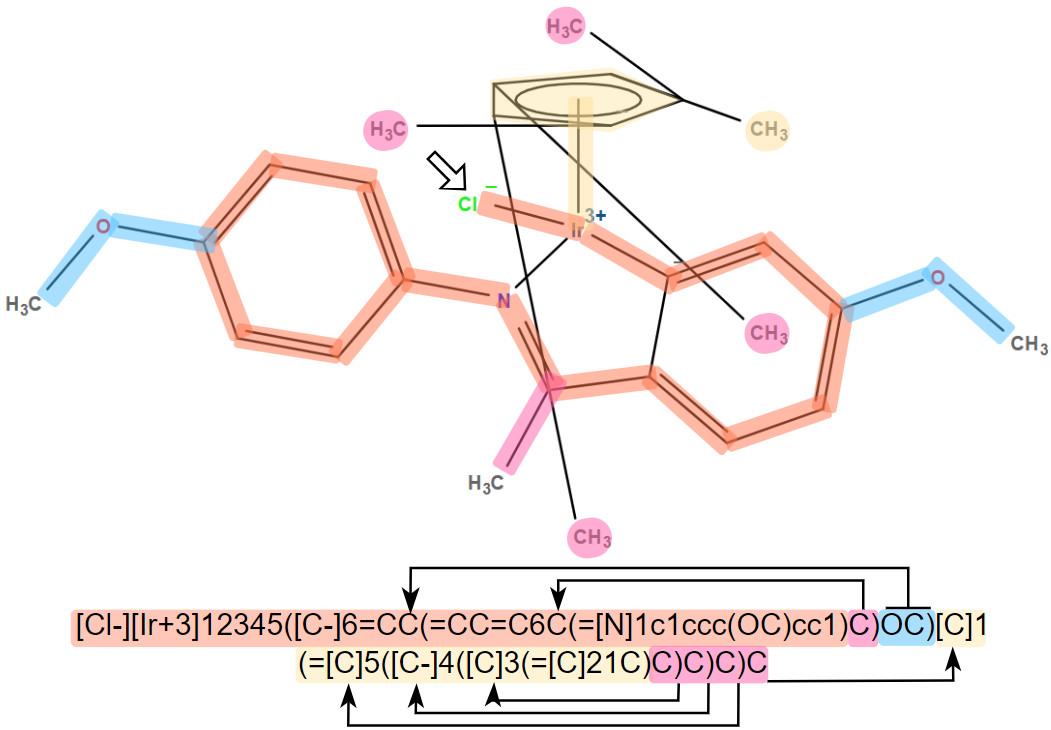
\includegraphics[width=.8\linewidth]{imagenes/resultados/moleculas/mol31_subrayao_malCanon.png}
  \caption{Canónico de OpenBabel}
\end{subfigure}%
\\
\\
\begin{subfigure}{.9\textwidth}
  \centering
  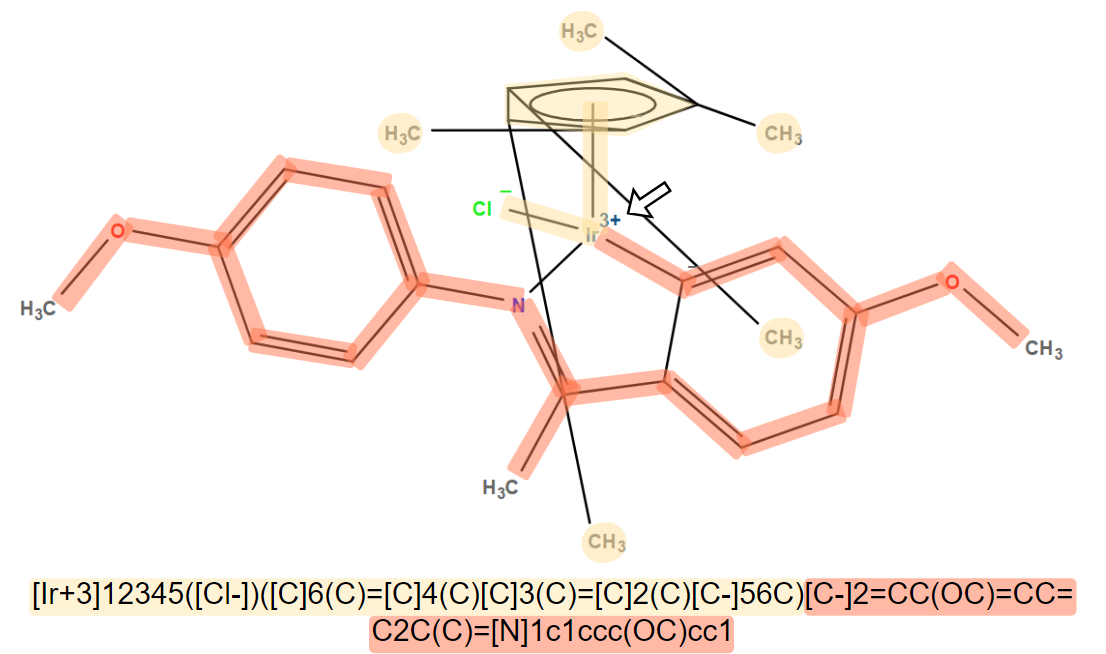
\includegraphics[width=.8\linewidth]{imagenes/resultados/moleculas/mol31_subrayao.png}
  \caption{Canónico propio}
\end{subfigure}
\caption{Correspondencia entre el SMILES canónico y la representación 2D de la molécula . \textbf{(a)} representación 2D usando mi algoritmo canónico con reordenación de ramas; y \textbf{(b)} usando mi algoritmo canónico con reordenación de ramas. La flecha indica el inicio del SMILES. Imagen de elaboración propia.}
\label{fig:smiles_vs_dibujo}
\end{figure}

\newpage

\section{Respresentación 2D}
Con respecto al cambio en la longitud de los enlaces, si bien no arregla el solapamiento de moléculas complejas, ya que esto requeriría de un cambio sustancial en el algoritmo de generación de coordenadas (si no, un rediseño completo), mejora en cierta medida la visibilidad de los enlaces. Para moléculas de este tipo donde todo aparece muy solapado y según las recomendaciones de los expertos, son preferibles estos resultados y que salga todo un poco más espaciado. En la Figura \ref{fig:bonds_longitud} se muestran los resultados para algunas moléculas del dataset.

\begin{figure}[h]
    \centering
    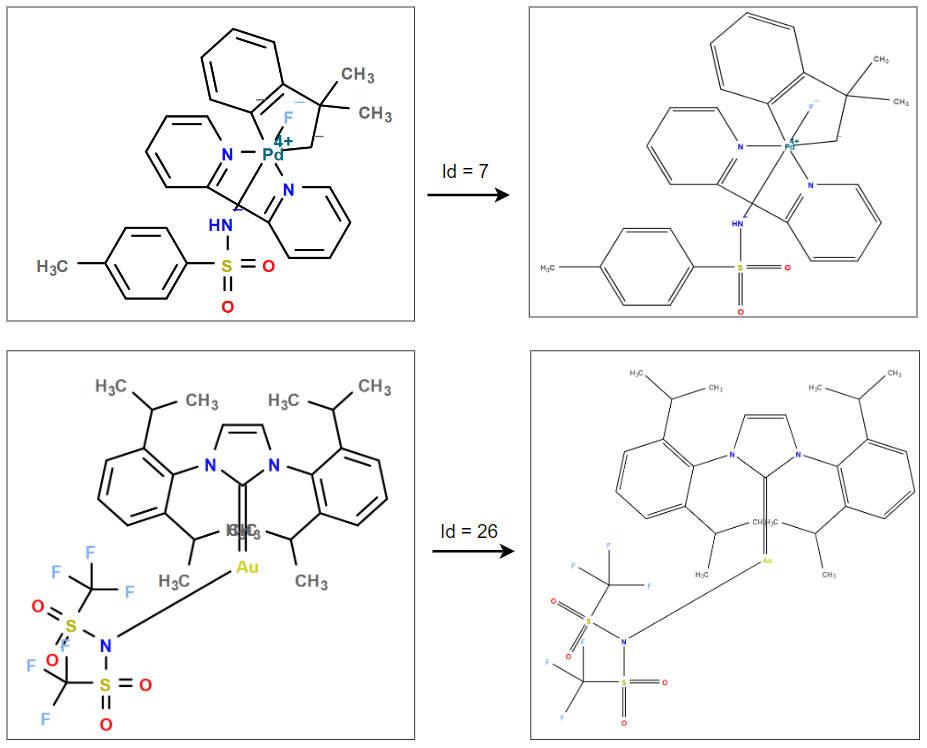
\includegraphics[scale=0.51]{imagenes/resultados/bond_longitud.png}
    \caption{Comparativa representación según la longitud de sus enlaces. A la izquierda las moléculas originales; a la derecha las moléculas con la longitud de enlaces aumentada.}
    \label{fig:bonds_longitud}
\end{figure}


En cuanto a la representación 2D de los Cp, se presenta en la Figura \ref{fig:evolucion_iron} la evolución en el proceso de dibujado mediante 3 fotos intermedias. Según lo discutido en la Sección \ref{implementacion:dibujado}, finalmente obtenemos el resultado buscado con la Figura \ref{fig:evolucion_iron_d}. En la Tabla \ref{tab:cps_dibujado} se muestran los resultados para las moléculas con estructuras Cp en nuestro dataset. Podemos apreciar una mejora en la representación considerable. Aquellas moléculas cuya representación no varíe apenas no se incluyen en este documento. Los ficheros `.svg' completos con todas las moléculas del dataset con el antes y el después están disponibles para su consulta en GitHub, por lo que se podrán inspeccionar y hacer zoom de manera detallada. Por su parte, los expertos han proporcionado las representaciones que ellos mismos harían a mano para algunas de las moléculas del dataset. En el Anexo \ref{apend:expertos_dibujos} se puede ver una comparativa entre los dibujos de los expertos, los resultados obtenidos y los de ambas bases de datos.

\begin{figure}[h]
\centering
\begin{subfigure}{.35\textwidth}
  \centering
  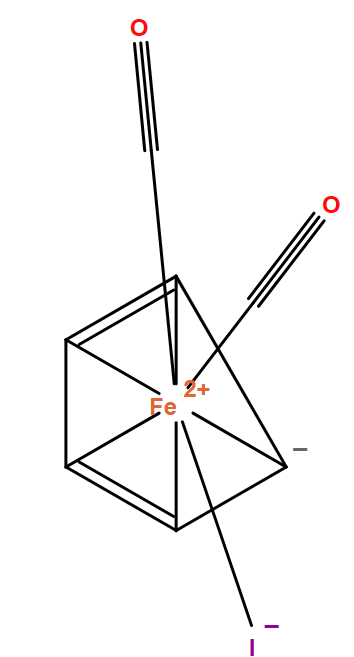
\includegraphics[width=.45\linewidth]{imagenes/resultados/evolucion_iron_a.png}
  \caption{}
\end{subfigure}%
\begin{subfigure}{.35\textwidth}
  \centering
  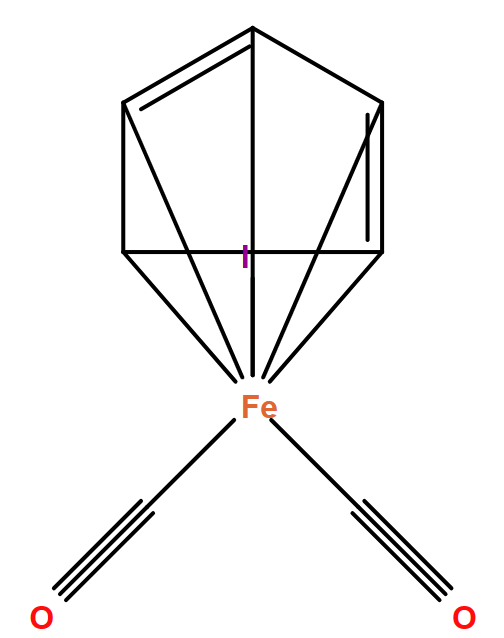
\includegraphics[width=.6\linewidth]{imagenes/resultados/evolucion_iron_b.png}
  \caption{}
\end{subfigure}%
\\
\begin{subfigure}{.35\textwidth}
  \centering
  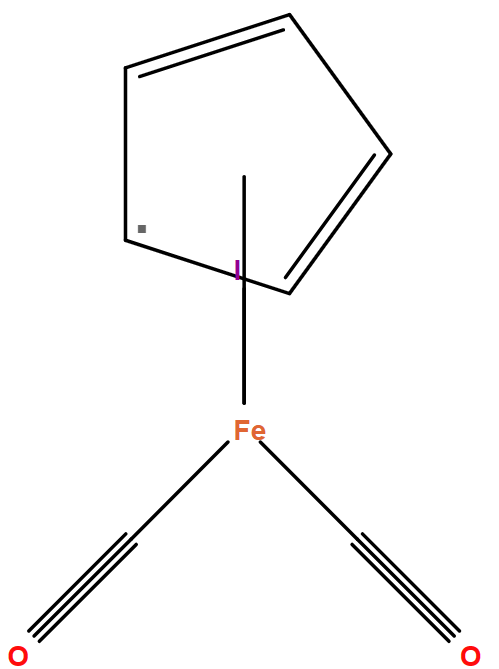
\includegraphics[width=.55\linewidth]{imagenes/resultados/evolucion_iron_c.png}
  \caption{}
\end{subfigure}%
\begin{subfigure}{.35\textwidth}
  \centering
  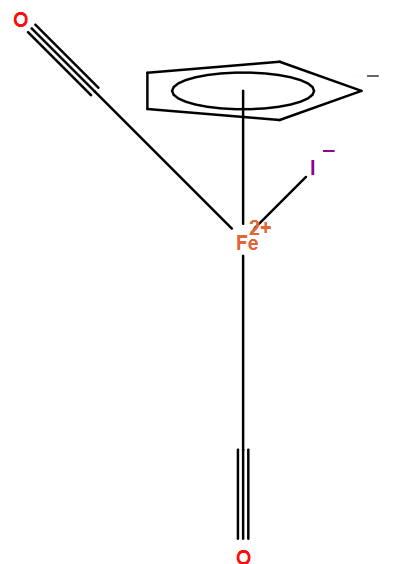
\includegraphics[width=.5\linewidth]{imagenes/resultados/moleculas/iron(II).png}
  \caption{}
  \label{fig:evolucion_iron_d}
\end{subfigure}%
\caption{Evolución durante la implementación del sistema de representación. Se muestra la molécula \textit{Dicarbonylcyclopentadienyliodoiron(II)} con Id 28 en el Anexo \ref{apend:pagina_tabla_intro_grande}. \textbf{(a)} original; \textbf{(b)} detección del Cp y modificación de la posición de los carbonos; \textbf{(c)} eliminación de enlaces y formación del polígono; y \textbf{(d)} polígono con perspectiva y curva central.}
\label{fig:evolucion_iron}
\end{figure}


% \newpage

\begin{longtable}{c>{\centering}m{5cm}>{\centering\arraybackslash}m{5.9cm}}
\caption{Resultados finales de los cambios en la representación para moléculas con Cp. Los Id hacen referencia al Anexo \ref{apend:pagina_tabla_intro_grande}.}\\

\toprule
 \textbf{Id} & \textbf{Original} & \textbf{Resultado} \\ \midrule
\endfirsthead

\multicolumn{3}{c}%
{{\bfseries \tablename\ \thetable{} -- Continuación de la página anterior}} \\
\toprule
\textbf{Id} & \textbf{Original} & \textbf{Resultado} \\ \midrule
\endhead

\hline \multicolumn{3}{r}{{Continúa en la siguiente página}} \\
\endfoot

\hline
\endlastfoot

% Mol 23
 23 & 
 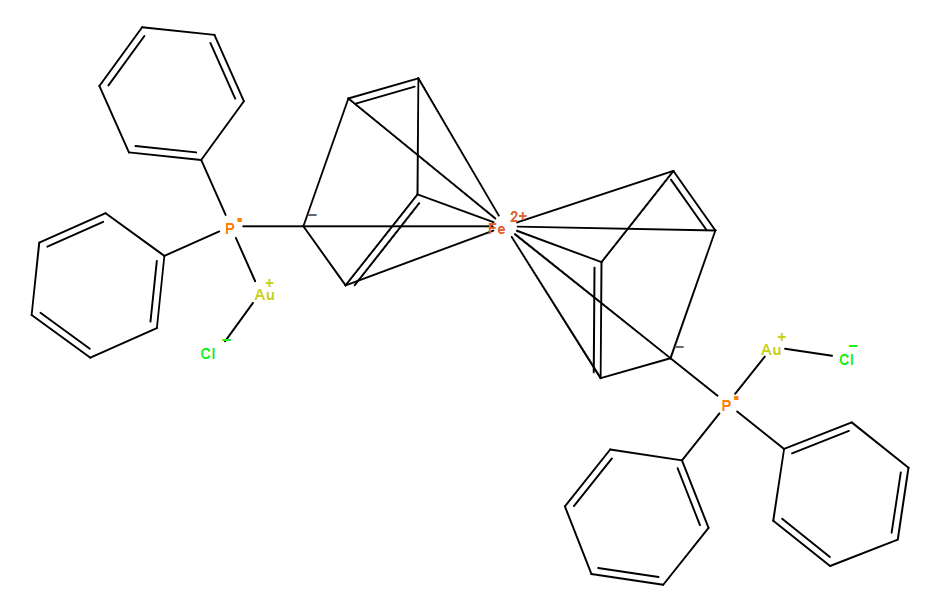
\includegraphics[width=4.3cm]{imagenes/resultados/cps/mol23_original.png} & 
 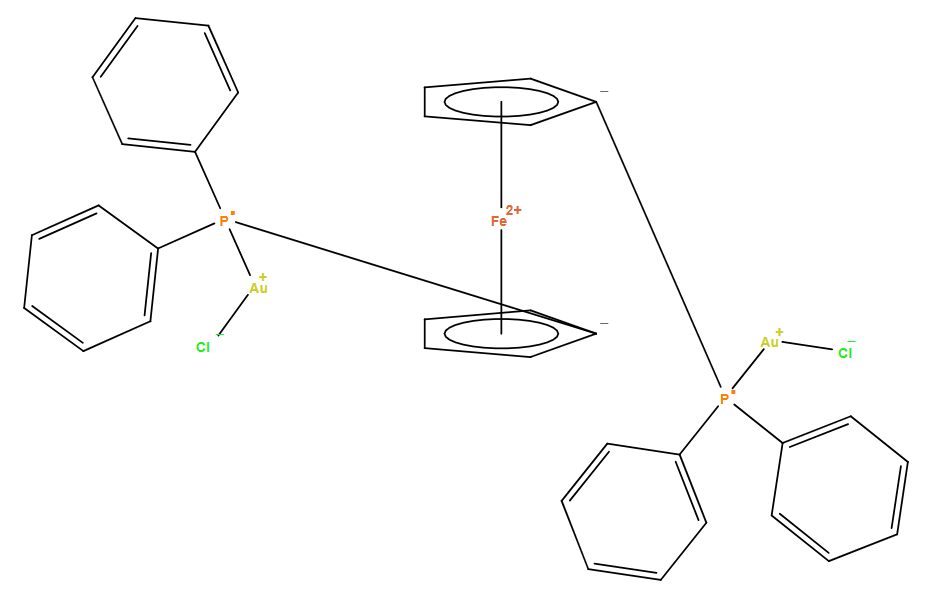
\includegraphics[width=4.3cm]{imagenes/resultados/cps/mol23_cp.png} \\
\midrule

% Mol 27
 27 &
 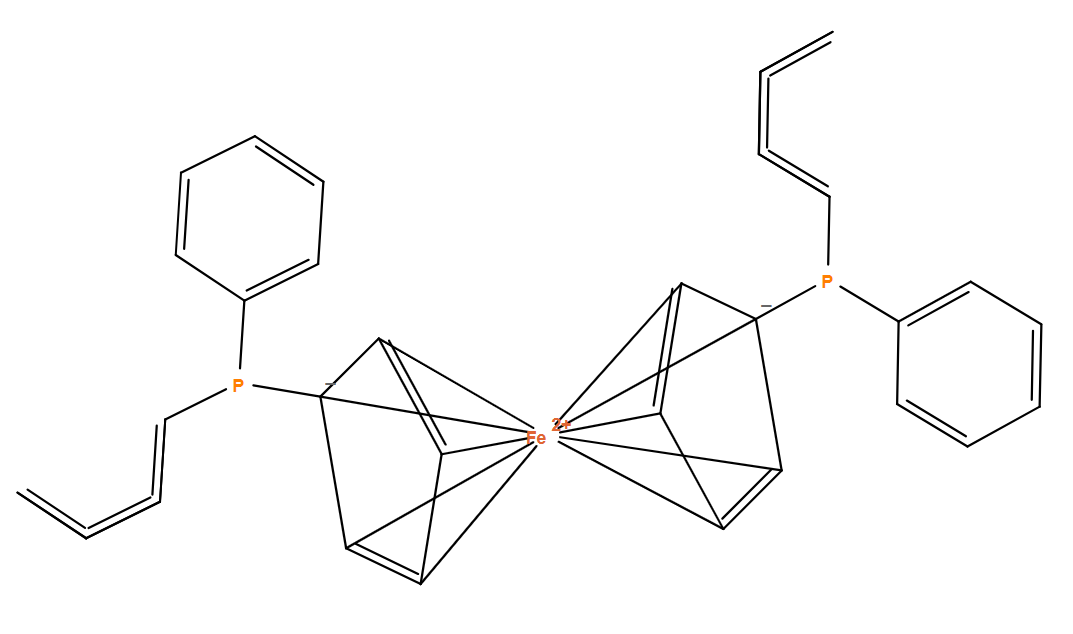
\includegraphics[width=4.3cm]{imagenes/resultados/cps/mol27_original.png} & 
 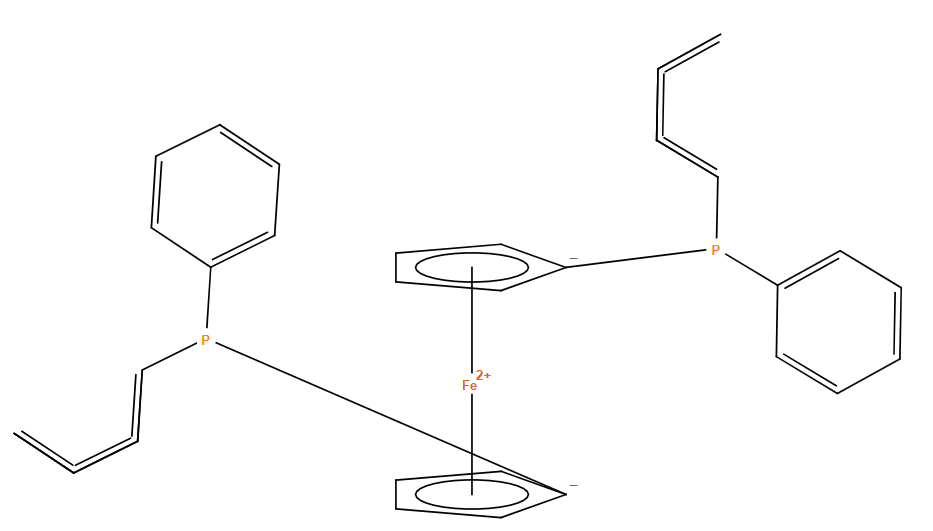
\includegraphics[width=4.3cm]{imagenes/resultados/cps/mol27_cp.png} \\
\midrule

% Mol 28
 28 &
 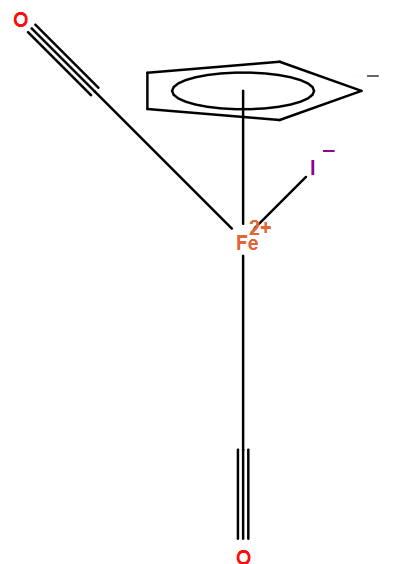
\includegraphics[width=2.5cm]{imagenes/resultados/moleculas/iron(II).png} & 
 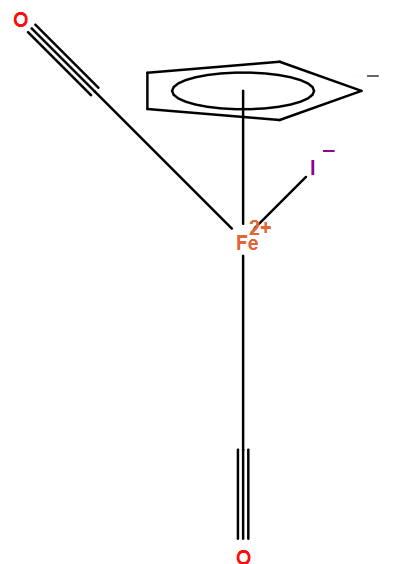
\includegraphics[width=2.5cm]{imagenes/resultados/moleculas/iron(II).png} \\
\midrule

% Mol 30
 30 &
 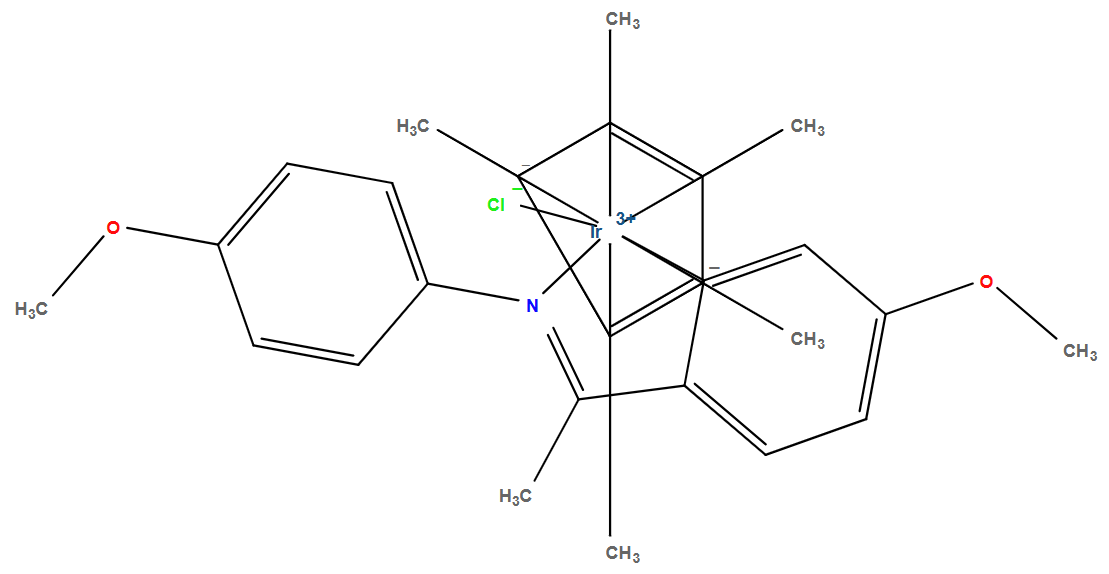
\includegraphics[width=4.3cm]{imagenes/resultados/cps/mol30_original.png} & 
 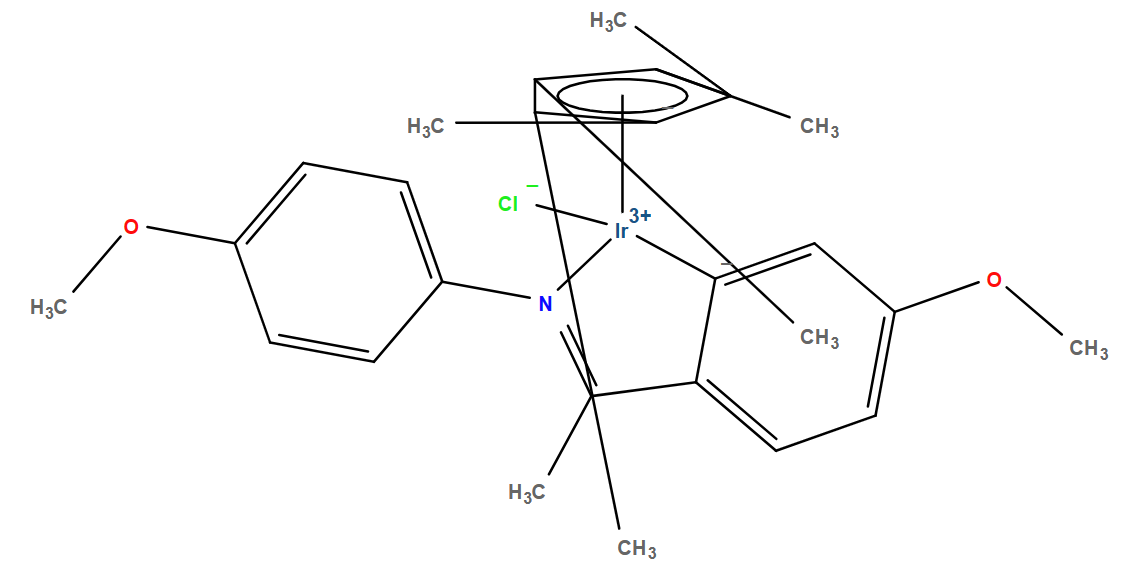
\includegraphics[width=4.3cm]{imagenes/resultados/cps/mol30_cp.png} \\
\midrule

% Mol 31
 31 &
 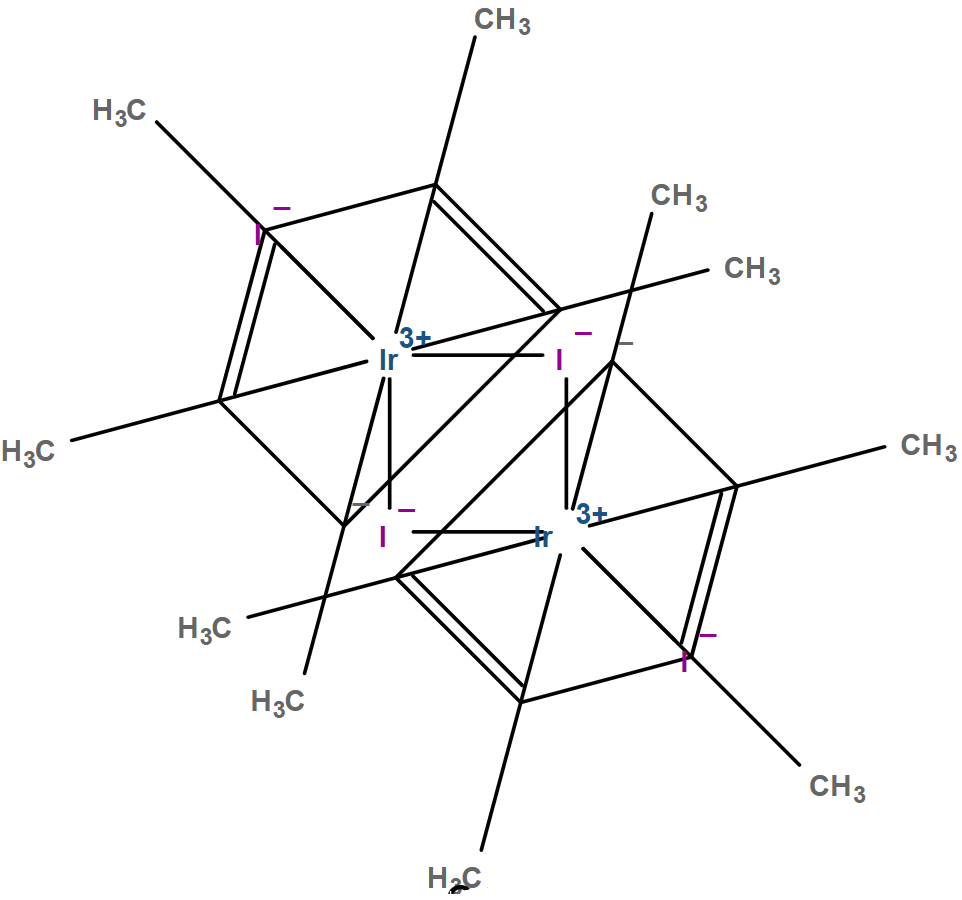
\includegraphics[width=4.3cm]{imagenes/resultados/cps/mol31_original.png} & 
 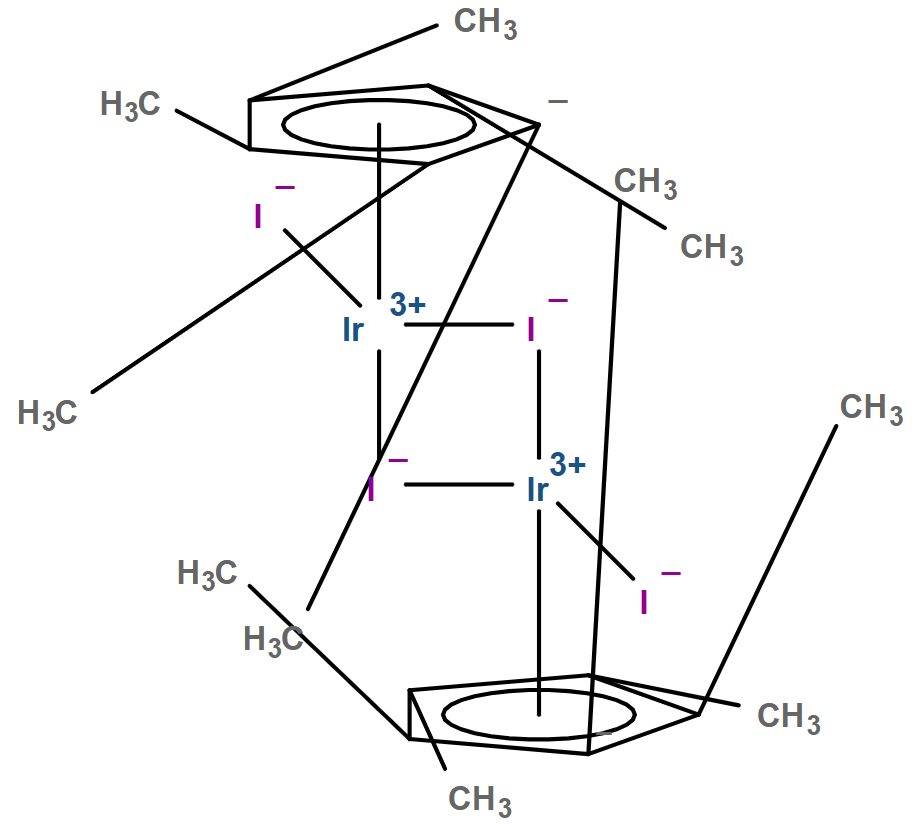
\includegraphics[width=4.3cm]{imagenes/resultados/cps/mol31_cp.png} 
% \midrule

\label{tab:cps_dibujado}
\end{longtable}




\subsection{Estructuras similares}
Destacar que la detección de estructuras Cp funciona de tal manera que no se limita estrictamente a enlaces de ligandos $\eta^{5}$-$C_{5}H_{5}$. Se es capaz de representar con el mismo estilo de dibujado ligandos de tipo $\eta^{x}$-$C_{x}H_{y}$, donde $[x \geq 3; 0 \leq y \leq x]$. Lo apreciamos en la siguiente Figura \ref{fig:n6_ligand_cp} con una estructura $\eta^{6}$-$C_{6}H_{4}$.

\begin{figure}[h!]
    \centering
    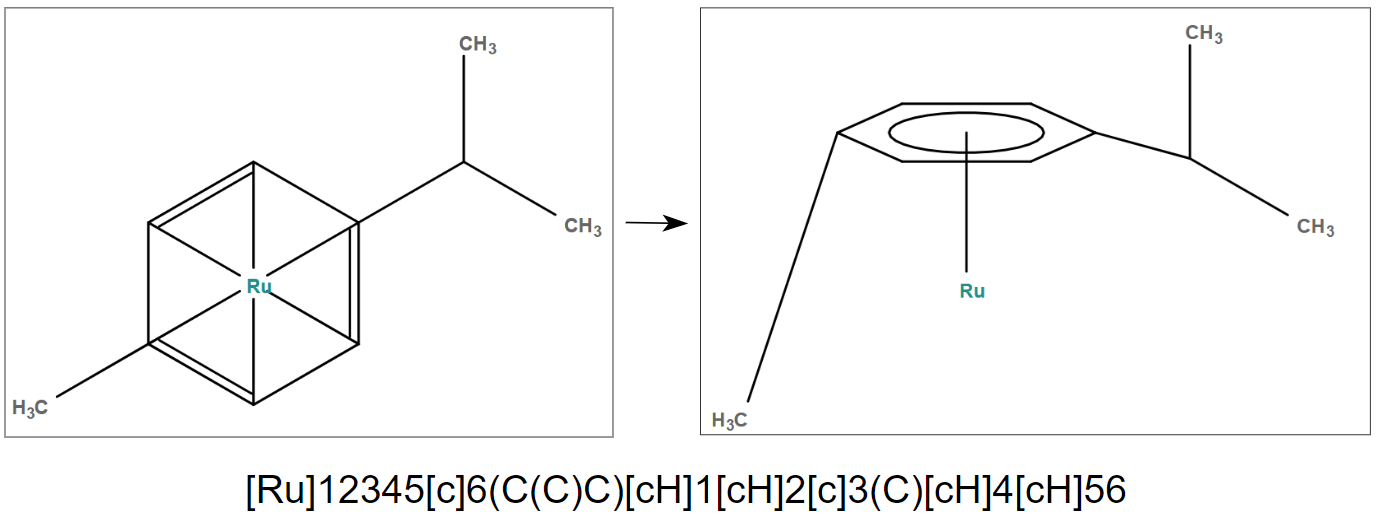
\includegraphics[scale=0.32]{imagenes/resultados/moleculas/Rutenio_n6_ligand_vs_original.png}
    \caption{Rutenio enlazado a un ligando `$\eta^{6}$-p-cyeme' junto con su cadena SMILES. Es una estructura que puede formar parte por ejemplo de moléculas experimentales bioactivas anti-cáncer \cite{rutenio_diimines_2018}.}
    \label{fig:n6_ligand_cp}
\end{figure}




\newpage

\subsection{Alias o abreviaciones}
Finalmente, comentar una de las opciones de representación gráfica que tiene disponible OpenBabel. Se trata de la generación de alias o abreviaturas. Esto consiste en sustituir una estructura completa por una etiqueta en texto con su nombre abreviado. Se utiliza para ello un fichero de datos que contiene un conjunto de abreviaciones estándar conocidas junto con su cadena SMILES equivalente. OpenBabel almacena estos datos en `\textit{/openbabel-3.1.1/data/superatom.txt}', de manera que modificando dicho fichero se pueden incluir estructuras de interés para su abreviación.

De este modo se ahorra un poco de espacio en las representaciones gráficas y se favorece su legibilidad evitando algunos casos de solapamientos, sobre todo causados por ciclos de benceno que son los que más ocupan. Esta funcionalidad se invoca con los parámetros por línea de órdenes `\textit{$--$genalias $-$xA}'. Se muestran algunas comparaciones, de las versiones sin alias y con alias en la Tabla \ref{tab:alias_vs_no_alias}.

\begin{table}[h!]
    \centering
    \begin{tabular}{c>{\centering}m{5cm}>{\centering\arraybackslash}m{5.9cm}}
        \toprule
        \textbf{Id} & \textbf{Versión normal} & \textbf{Versión con abreviaciones} \\
        \midrule
        6 &
        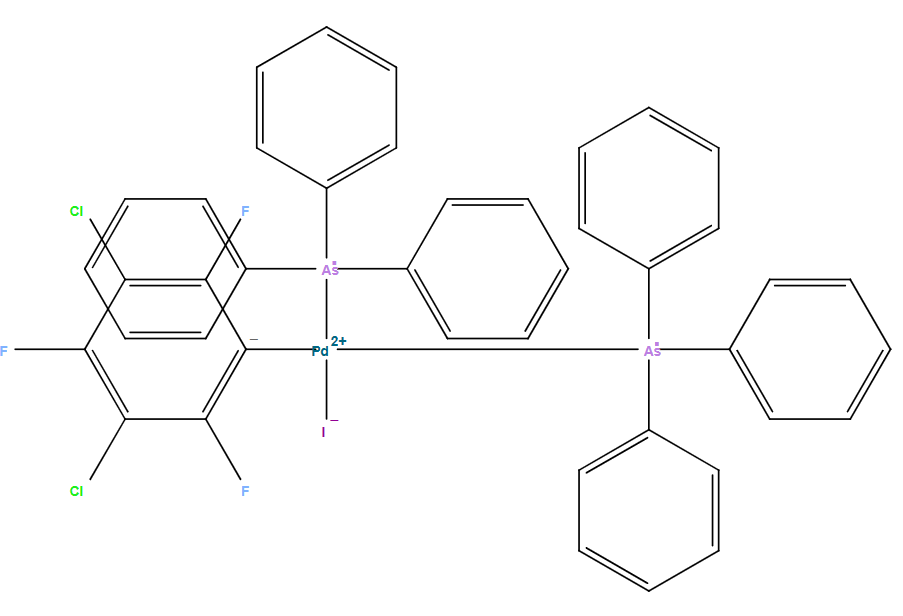
\includegraphics[width=4.7cm]{imagenes/resultados/moleculas/mol6.png} & 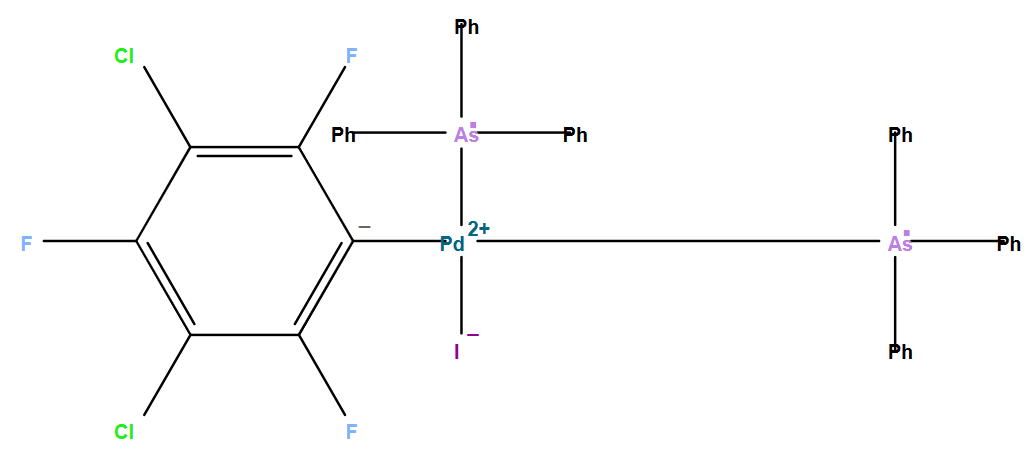
\includegraphics[width=4.7cm]{imagenes/resultados/moleculas/mol6_ALIAS.png} \\
        \midrule
        9 &
       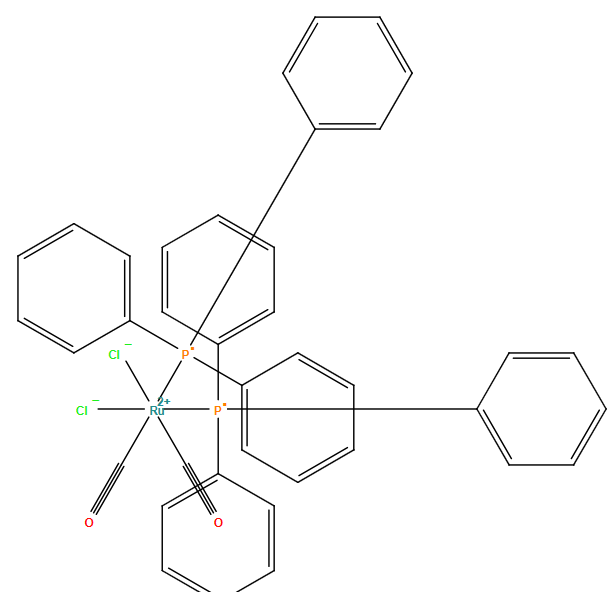
\includegraphics[width=4.2cm]{imagenes/resultados/moleculas/mol9.png} & 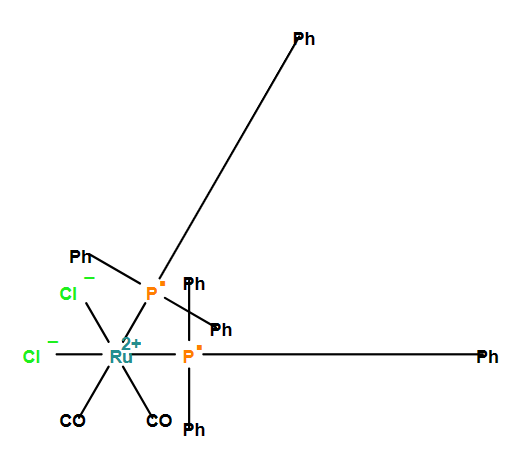
\includegraphics[width=4.2cm]{imagenes/resultados/moleculas/mol9_alias.png} \\ 
        \midrule
        28 &
        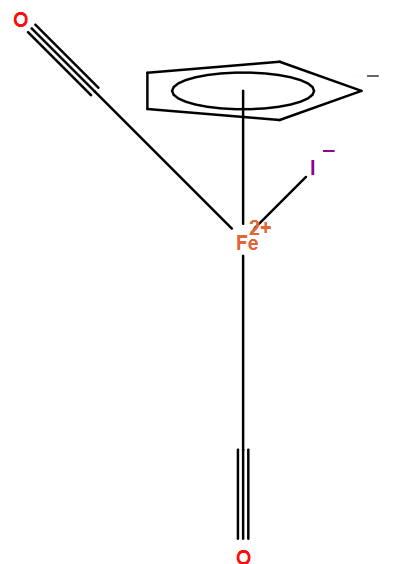
\includegraphics[width=3cm]{imagenes/resultados/moleculas/iron(II).png} & 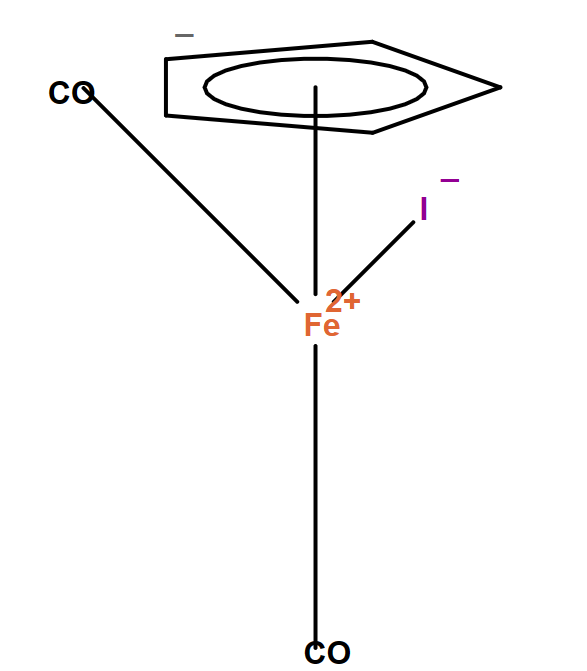
\includegraphics[width=3.5cm]{imagenes/resultados/moleculas/iron(II)_alias.png} \\
        \bottomrule
        \end{tabular}
    \caption{Comparativa de algunas representaciones 2D entre su versión normal y su alternativa usando abreviaciones. Los Id hacen referencia al Anexo \ref{apend:pagina_tabla_intro_grande}.}
    \label{tab:alias_vs_no_alias}
\end{table}



\newpage



% ------------------------------ Pruebas ----------------------------------
\section{Pruebas} \label{pruebas}
El propio proyecto de OpenBabel ya trae consigo un entorno de pruebas, que se gestiona a través del ejecutable 'test\_runner.exe'. Según los parámetros que le pases al programa, se ejecutará un test u otro. Dichos tests pueden incluso albergar otros tests más específicos dentro. La ejecución de un test concreto sigue este esquema: 
\begin{center}
    \textit{test\textunderscore runner \textless nombreTest\textgreater  \textless numeroTest\textgreater}    
\end{center}

Un ejemplo de llamada al test ``conversion", que es un test único sería: \textit{test\_runner.exe conversion}. Con la llamada \textit{test\_runner.exe regressiontest 225} se estaría ejecutando el test número 225 especificado en regressiontest.cpp. A la hora de añadir nuevos ficheros de testing hay que seguir una serie de indicaciones y utilizar una sintaxis especial para determinar si el test es correcto o no. Esto se describe en la guía para desarrolladores de la página oficial de OpenBabel\footnote{\url{https://openbabel.org/docs/current/Contributing/Testing.html}}\footnotecomma\footnote{\url{https://open-babel.readthedocs.io/en/latest/Contributing/Testing.html}} (en el Anexo \ref{apend:manual} se describe como añadir nuevos tests).

Dicho esto, la mayoría de tests que se han realizado son tests funcionales completos. Hacer un test de unidad de según que métodos es complicado ya que necesitan una serie de parámetros y variables que se van creando sobre la marcha en multitud de métodos previos. El fichero de pruebas creado específicamente para el proyecto se llama ``canonogmtest.cpp'' y tiene la siguiente estructura:
\vspace{0.2cm}
\dirtree{%
    .1 test\_runner.cpp\DTcomment{fichero main gestor de pruebas}.
    .2 canonogmtest.cpp\DTcomment{fichero main de pruebas para el proyecto}.
    .3 SelectCanonMetal\DTcomment{prueba 1}.
    .3 RandomCanonStandardLabels\DTcomment{prueba 2}.
    .3 RandomCanonCanonicalLabels\DTcomment{prueba 3}.
    .3 CanonOverCanon\DTcomment{prueba 4}.
    .3 DrawDoubleCpTest\DTcomment{prueba 5}.
    .2 Otros .cpp de pruebas creados por OpenBabel.
    .3 regressiontest.cpp.
    .3 ringtest.cpp.
    .3 invalidsmiles.cpp.
    .3 conversion.cpp.
    .3 ....
    .3 ....
}

En el GitHub del proyecto se pueden consultar los ficheros de salida que resultaron de la ejecución de las pruebas (las que tengan alguna salida). Este proceso de testing, tal como indico en la Sección \ref{aplicacion_metod}, se realizaba de manera frecuente para comprobar si los resultados iban siendo los esperados. A continuación se describen las pruebas llevadas a cabo:

\begin{itemize}
    \item \textbf{Test unitario}
    \begin{itemize}
        \item \textbf{SelectCanonMetal}: comprueba que el método \textit{OBMol2Cansmi:: SelectRootAtomOgm} funciona correctamente eligiendo el átomo adecuado de entre todos los átomos para moléculas que contengan algún metal. Los SMILES a comprobar se cargan de un fichero, junto con el identificador del átomo que se debería seleccionar. El test es válido si el identificador cargado y el que devuelve el método coinciden.
    \end{itemize}

    \item \textbf{Tests funcionales}
    \begin{itemize}
        \item \textbf{RandomCanonStandardLabels}: comprueba la consistencia de la nomenclatura canónica para la forma estándar. Se toman los SMILES de prueba desde un fichero y se obtienen unos SMILES sinónimos de manera aleatoria para la misma molécula. Tanto el SMILES original como el randomizado se canonizan a su forma estándar. El test es válido si ambos canónicos obtenidos coinciden. Por lo general, teniendo en cuenta lo discutido en la Sección \ref{implementacion:canonizado} es normal que el test falle.

        \item \textbf{RandomCanonCanonicalLabels}: comprueba la consistencia de la nomenclatura canónica para la forma canónica. Se toman los SMILES de prueba desde un fichero y se obtienen unos SMILES sinónimos de manera aleatoria para la misma molécula. Tanto el SMILES original como el randomizado se canonizan a su forma canónica. El test es válido si ambos canónicos obtenidos coinciden.
    
        \item \textbf{CanonOverCanon}: comprueba la consistencia de la nomenclatura canónica. Se toman los SMILES de prueba desde un fichero y se canonizan. A esos SMILES canonizados, se les vuelve a aplicar el algoritmo. Con este test se quiere verificar que sucesivas aplicaciones del algoritmo no degeneren el resultado o haya una vaivén de los átomos, como sería el caso de la Figura \ref{fig:canonOverCanon}. El test es válido si ambos resultados coinciden.

        \begin{figure}[h!]
            \centering
            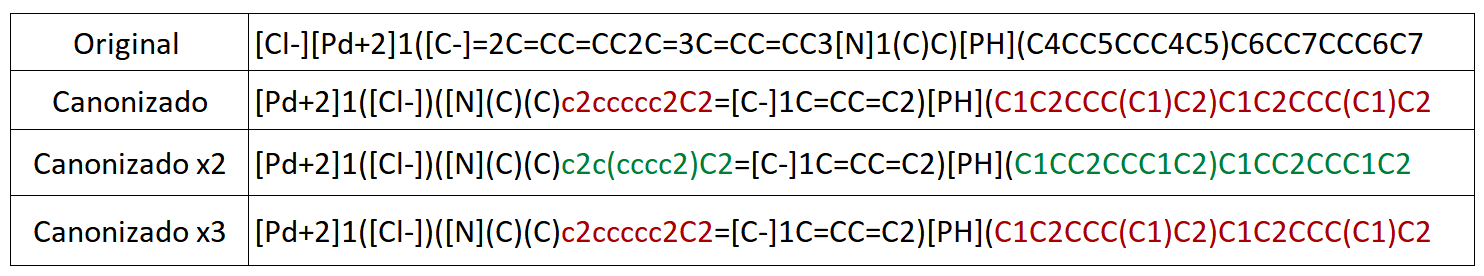
\includegraphics[scale=0.3]{imagenes/resultados/pruebas/canonOverCanon.png}
            \caption{Ejemplo de una canonización imperfecta. Se muestra el SMILES original, y los SMILES canónicos tras haber aplicado 1, 2 y 3 veces el algoritmo sobre el anterior resultado respectivamente. Esto no ocurre con ninguna de las moléculas probadas.}
            \label{fig:canonOverCanon}
        \end{figure}
    
        \item \textbf{DrawDoubleCpTest}: comprueba si los algoritmos de dibujado para moléculas con múltiples Cp se aplican correctamente. Se introduce una molécula sabida de antemano que contiene varias de estas estructuras y se realiza la conversión. El test en sí tiene es válido si el proceso de conversión tiene éxito. Dado que analizar de manera automática el resultado de una representación gráfica en formato .svg no es tarea fácil, hay que verificar si el resultado es el esperado de acuerdo a lo descrito en la Sección \ref{implementacion:dibujado} de manera manual.
    
    \end{itemize}
\end{itemize}

Se han ejecutado también otros tests útiles como el \textit{invalidsmiles} para comprobar que OpenBabel rechazaba SMILES incorrectos. Decir que para los tests \textit{RandomCanonStandardLabels}, \textit{RandomCanonCanonicalLabels} y \textit{CanonOverCanon} se han usado datasets relativamente grandes, de aproximadamente 1000 moléculas incluyendo química orgánica general y las moléculas nuestras propias de organometálica. Para todas ellas, salvo 6 excepciones de estereoquímica con compuestos cis/trans, el test se cumple. Notar que la nomenclatura implementada sólo se aplica a las moléculas pertenecientes a la organometálica, por lo que para compuestos orgánicos normales se aplica el algoritmo previo de OpenBabel. Se han añadido entonces para comprobar que no se alteraba el comportamiento por defecto. Las otras dos pruebas son mucho más selectivas y específicas, por lo que se han aplicado a nuestro dataset simplemente.

